\usetikzlibrary{calc,fit, positioning}


\begin{figure}[t]
	\centering
\begin{adjustbox}{width=\columnwidth}
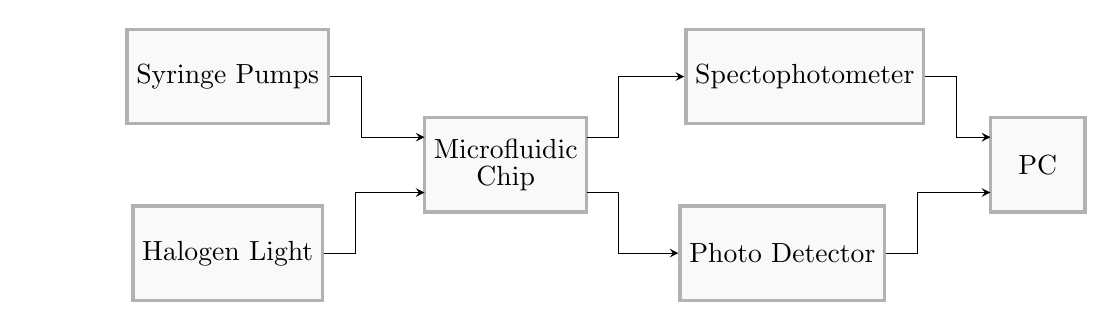
\begin{tikzpicture}[
%square node outer loop
squarednodeo/.style={rectangle, draw=white!28, fill=white!25, very thick, minimum size=2mm},
%square node intermediate loop
squarednodei/.style={rectangle, draw=red!35, fill=red!25, very thick, minimum size=8mm},
%square node inner loop
squarednodeii/.style={rectangle, draw=orange!25, fill=orange!20, very thick, minimum size=12mm},
dot/.style={circle, fill=black,	minimum size=1mm, inner sep=0mm, outer sep=0mm,
	node contents={}
},
squarednodefc/.style={rectangle, draw=gray!60, fill=gray!5, very thick, minimum size=12mm},
dot/.style={circle, fill=black,	minimum size=1mm, inner sep=0mm, outer sep=0mm,
	node contents={}
},
squarednodemux/.style={rectangle, draw=black, fill=black, very thick, minimum width=0.5mm, minimum height=30mm},
]
\node (start) [draw=none,fill=none] {};
\node[squarednodefc] (pp) [right=of start]{\shortstack{Syringe Pumps}};
\node[squarednodefc] (hl) [below=of pp]{\shortstack{Halogen Light}};

\node[squarednodefc,outer sep=0pt,right=2.5cm of $(pp)!.5!(hl)$](mc){\shortstack{Microfluidic \\ Chip}};

\node[squarednodefc] (sp) [right=4.5cm of pp]{\shortstack{Spectophotometer}};
\node[squarednodefc] (pd) [right=4.5cm of hl]{\shortstack{Photo Detector}};

\node[squarednodefc,outer sep=0pt,right=2.5cm of $(sp)!.5!(pd)$](pc){\shortstack{PC}};

\draw[- stealth] (pp.east) |- ++ (0.4,0) |- ([yshift= 10pt]mc.west);
\draw[- stealth] (hl.east) |- ++ (0.4,0) |- ([yshift= -10pt]mc.west);

\draw[- stealth] ([yshift= 10pt]mc.east) |- ++ (0.4,0) |- (sp.west);
\draw[- stealth] ([yshift= -10pt]mc.east) |- ++ (0.4,0) |- (pd.west);

\draw[- stealth] (sp.east) |- ++ (0.4,0) |- ([yshift= 10pt]pc.west);
\draw[- stealth] (pd.east) |- ++ (0.4,0) |- ([yshift= -10pt]pc.west);


%\node[squarednodei] (IMU) [right=of start]{IMU};
%\node[squarednodei] (Mocap) [below=3mm of IMU]{Mocap};

%\node (temp)[draw=none,fill=none, above=1mm of IMU] {};
%\node[squarednodei] (VO) [above=3mm of IMU]{VO};
%\node[squarednodei] (GPS) [above=3mm of VO]{GPS};
%\node[squarednodemux] (mux) [right= 30mm of temp] {};p
%\node[squarednodeii] (use) [right=of mux]{\shortstack{Unconstrained \\ State Estimation}};
%\node[squarednodeo] (cse) [right=of use]{\shortstack{Constrained\\State Estimation}};

%\draw [- stealth] (use.east) -- (cse);
%\draw [- stealth] (cse.east) -- (ctrl);
%\draw [- stealth] (mux) -- (use);

% Switch IMU
%\node (isw) [dot, right=of IMU]{};
%\draw (IMU.east) -- (isw.west);
%\node (osw) [dot, right=2mm of isw]{};
%\draw(3.1,0)-- +(-25:0.3);
%\draw[- stealth] (osw.north) |- ++ (0,0) |- ([yshift=-11pt]mux.west);

% Switch Mocap
%\node (isw1) [dot, right=of Mocap]{};
%\draw (Mocap.east) -- (isw1.west);
%\node (osw1) [dot, right=2mm of isw1]{};
%\draw(3.24,-1.11)-- +(-25:0.3);
%\draw[- stealth] (osw1.north) |- ++ (0,0) |- ([yshift=-32pt]mux.west);

% Switch VO
%\node (isw2) [dot, right=of VO]{};
%\draw (VO.east) -- (isw2.west);
%\node (osw2) [dot, right=2mm of isw2]{};
%\draw(3.08,1.14)-- +(-25:0.3);
%\draw[- stealth] (osw2.east) |- ++ (0.3,0) |- ([yshift=12pt]mux.west);

% Switch IMU
%\node (isw3) [dot, right=of GPS]{};
%\draw (GPS.east) -- (isw3.west);
%\node (osw3) [dot, right=2mm of isw3]{};
%\draw(3.1,2.28)-- +(-25:0.3);
%\draw [- stealth] (osw3.east) |- ++ (0.3,0) |- ([yshift=33pt]mux.west);

% Labels
%\put (70, 68) {$\tilde{\vect{p}}$};
%\put (70, 36) {$\tilde{\vect{p}},\tilde{\vect{v}}$};
%\put (70,2) {$\tilde{\vect{a}},\tilde{\vect{\omega}}$};
%\put (70, -30) {$\tilde{\vect{p}}$};

%\put (150, 22) {$\measR{i}$};
%\put (253, 22) {$\stateRest{i}$};
%\put (355, 22) {$\stateRproj{i}$};

\end{tikzpicture}
 \end{adjustbox}
\caption{The complete block diagram of the experimental setup used for the device microptofluidic characterization }
\label{fig:block-diagram}
\end{figure}
